\documentclass{beamer}

\mode<presentation> {

%\usetheme{default}
%\usetheme{AnnArbor}
%\usetheme{Antibes}
%\usetheme{Bergen}
%\usetheme{Berkeley}
%\usetheme{Berlin}
%\usetheme{Boadilla}
%\usetheme{CambridgeUS}
%\usetheme{Copenhagen}
%\usetheme{Darmstadt}
%\usetheme{Dresden}
%\usetheme{Frankfurt}
%\usetheme{Goettingen}
%\usetheme{Hannover}
%\usetheme{Ilmenau}
%\usetheme{JuanLesPins}
%\usetheme{Luebeck}
\usetheme{Madrid}
%\usetheme{Malmoe}
%\usetheme{Marburg}
%\usetheme{Montpellier}
%\usetheme{PaloAlto}
%\usetheme{Pittsburgh}
%\usetheme{Rochester}
%\usetheme{Singapore}
%\usetheme{Szeged}
%\usetheme{Warsaw}


%\usecolortheme{albatross}
%\usecolortheme{beaver}
%\usecolortheme{beetle}
%\usecolortheme{crane}
%\usecolortheme{dolphin}
%\usecolortheme{dove}
%\usecolortheme{fly}
%\usecolortheme{lily}
%\usecolortheme{orchid}
%\usecolortheme{rose}
%\usecolortheme{seagull}
%\usecolortheme{seahorse}
%\usecolortheme{whale}
%\usecolortheme{wolverine}

%\setbeamertemplate{footline} % To remove the footer line in all slides uncomment this line
%\setbeamertemplate{footline}[page number] % To replace the footer line in all slides with a simple slide count uncomment this line

%\setbeamertemplate{navigation symbols}{} % To remove the navigation symbols from the bottom of all slides uncomment this line
}

\usepackage{graphicx} % Allows including images
\usepackage{booktabs} % Allows the use of \toprule, \midrule and \bottomrule in tables
\usepackage{amsfonts}
\usepackage{mathrsfs}
\usepackage{amsmath,amssymb,graphicx}

%----------------------------------------------------------------------------------------
%	TITLE PAGE
%----------------------------------------------------------------------------------------

\title["12.1"]{12.1: The Simple Linear and Logistic Regression Models}

\author{Taylor} 
\institute[UVA] 
{
University of Virginia \\
\medskip
\textit{} 
}
\date{} 

\begin{document}
%----------------------------------------------------------------------------------------

\begin{frame}
\titlepage 
\end{frame}
%----------------------------------------------------------------------------------------
\begin{frame}
\frametitle{Introduction}

So far we've been assuming that we have a random sample (independent and \emph{identically distributed})
\[
Y_1, \ldots, Y_n \overset{iid}{\sim} \text{something}(\theta)
\]

\pause
Now we'll talk about when our data are still mutually independent, but not \emph{identically distributed}
\[
Y_1 \sim \text{something}_1(\theta), \ldots, Y_n \sim \text{something}_n(\theta)
\]
\pause

We still need to fit/learn parameters, and we'll also observe predictors/inputs/covariates $X_1, \ldots, X_n$.
\end{frame}

%----------------------------------------------------------------------------------------
\begin{frame}
\frametitle{Introduction}

We want to develop a framework for modelling a \emph{probabilistic} dependence between a \textbf{dependent response} ($Y$) and an \textbf{independent, explanatory predictor} ($X$). The general form of our model is 
\[
Y = f(x) + \epsilon
\]
where $f(\cdot)$ is a \emph{deterministic} function and $\epsilon$ is a random error (random variable).


\end{frame}
%----------------------------------------------------------------------------------------
\begin{frame}
\frametitle{Introduction}

How do we get an idea for what $f(\cdot)$ should be? Typically we plot $x_1, \ldots, x_n$ against $y_1, \ldots, y_n$. This is called a \textbf{scatterplot}.
\newline

Also, theoretical/scientific justification is often necessary/advised.

\end{frame}
%----------------------------------------------------------------------------------------
\begin{frame}
\frametitle{Simple Linear Regression}

When there looks to be a linear relationship, we can use this model, the \textbf{simple linear regression model}.
\[
Y = \beta_0 +\beta_1 x + \epsilon
\]
and 
\begin{enumerate}
\item $\epsilon \sim \mathcal{N}(0, \sigma^2)$ (does not depend on what $x$ is)
\end{enumerate}

\end{frame}
%----------------------------------------------------------------------------------------
\begin{frame}
\frametitle{Simple Linear Regression}

Remember we think of all the $X$ data and the coefficients as constants...

\begin{align*}
E[Y] &= E[\beta_0 +\beta_1 x + \epsilon ] \\
&= \beta_0 +\beta_1 x + E[\epsilon] \\
&= \beta_0 + \beta_1x 
\end{align*}

\begin{align*}
V[Y] &= V[\beta_0 +\beta_1 x + \epsilon ] \\
&= V[\epsilon] \\
&= \sigma^2
\end{align*}

So now $Y$ is still normal, but has a mean that changes with an input
\end{frame}
%----------------------------------------------------------------------------------------
\begin{frame}
\frametitle{Simple Linear Regression}

\begin{center}
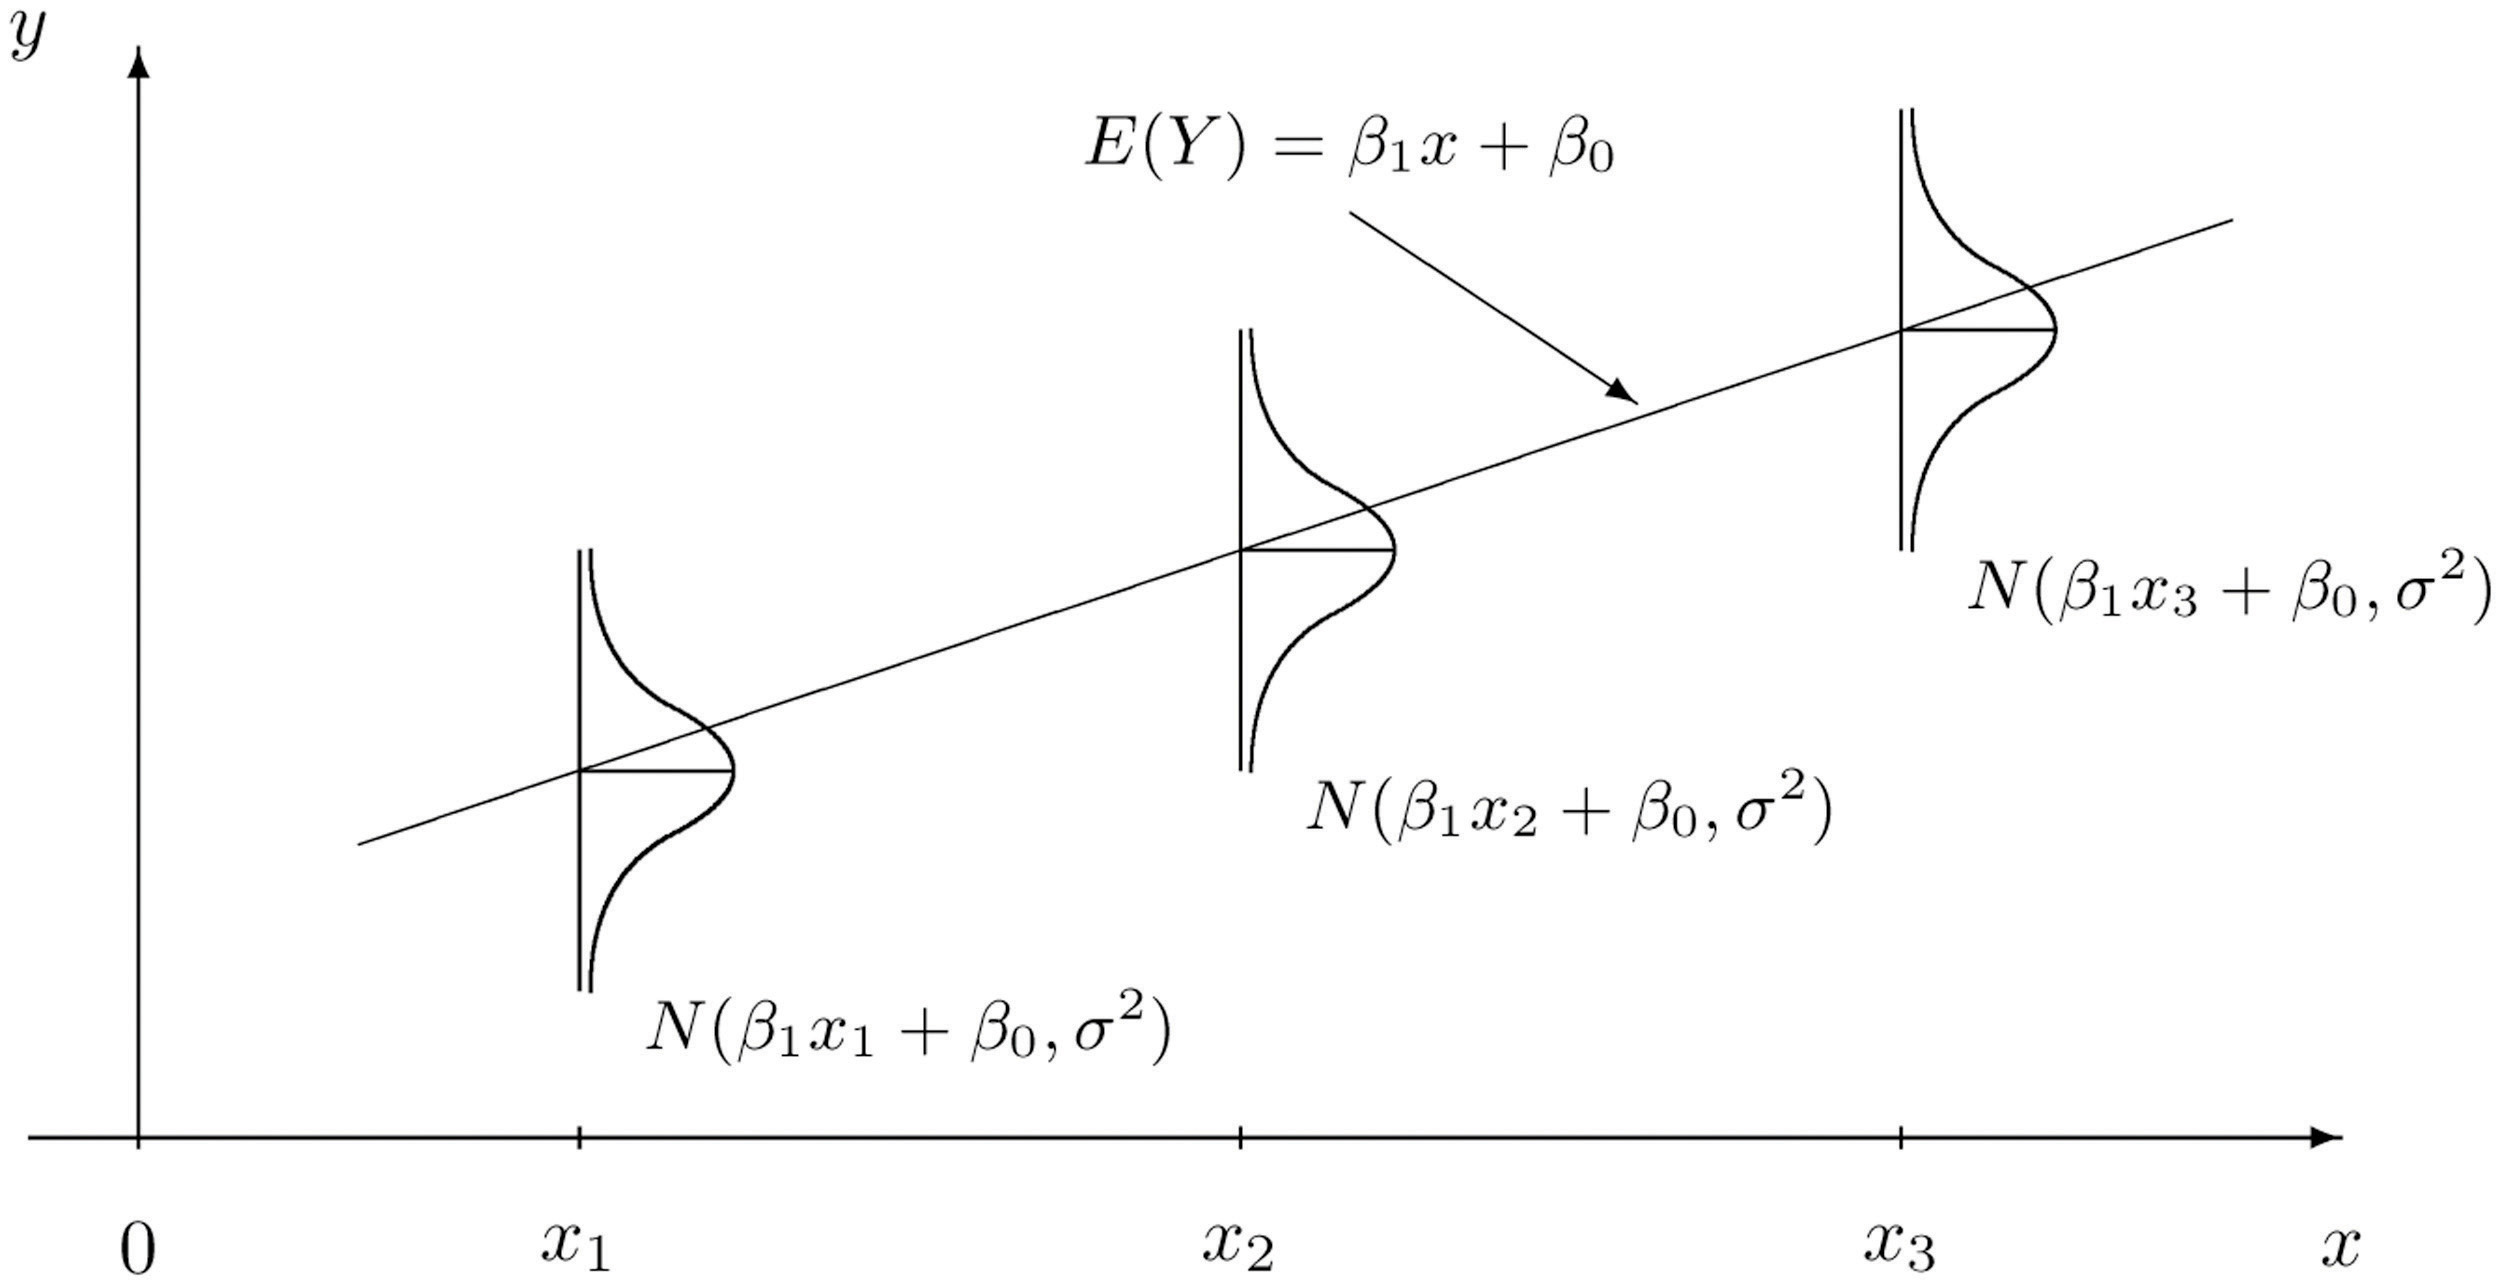
\includegraphics[width=90mm]{/home/t/UVa/all_teaching/3120_slides/12/12.1/pics/slr.jpg}
\end{center}

So if I tell you $X = 4$, you can answer questions like what's the probability that $Y > 5$...
\newline

Also, keep in mind $\beta_0$, $\beta_1$ and $\sigma^2$ are population parameters...we don't know them yet.

\end{frame}
%----------------------------------------------------------------------------------------
\begin{frame}
\frametitle{Simple Linear Regression}

If our scatterplot looks like this:
\begin{center}
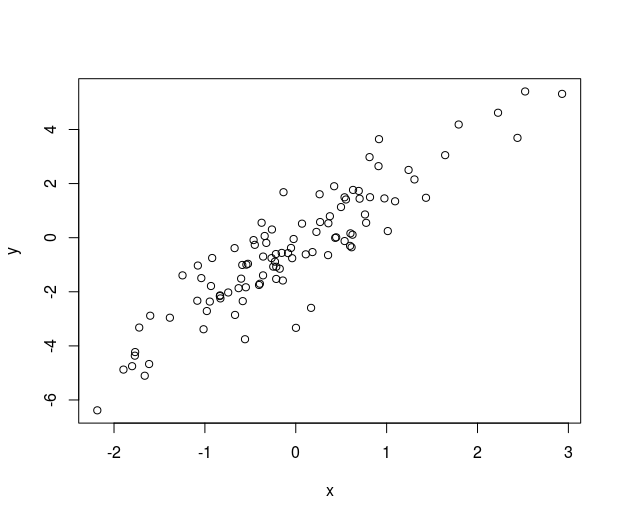
\includegraphics[width=70mm]{/home/t/UVa/all_teaching/3120_slides/12/12.1/pics/Rplot.png}
\end{center}

then we suspect a good model fit. The output of the regression software will be the estimates $\hat{\beta}_0$, $\hat{\beta}_1$ and $\hat{\sigma}^2$.


\end{frame}
%----------------------------------------------------------------------------------------
\begin{frame}
\frametitle{Simple Linear Regression}

If our scatterplot looks like this:
\begin{center}
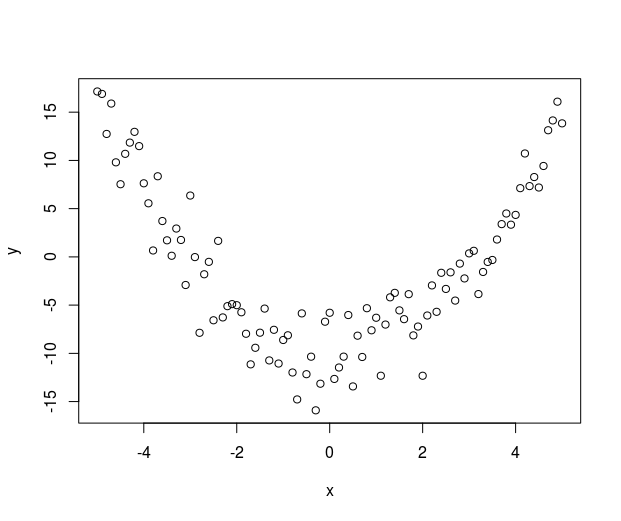
\includegraphics[width=70mm]{/home/t/UVa/all_teaching/3120_slides/12/12.1/pics/Rplot01.png}
\end{center}

then we shouldn't just plug in the x and y data into the regression software. What can we do?


\end{frame}

%----------------------------------------------------------------------------------------
\begin{frame}
\frametitle{Simple Linear Regression}

Instead of plugging in the data $\{x_i,y_i\}$, we should plug in the \emph{ transformed} data $\{x_i^2,y_i\}$! Here is the scatterplot of the transformed data:
\begin{center}
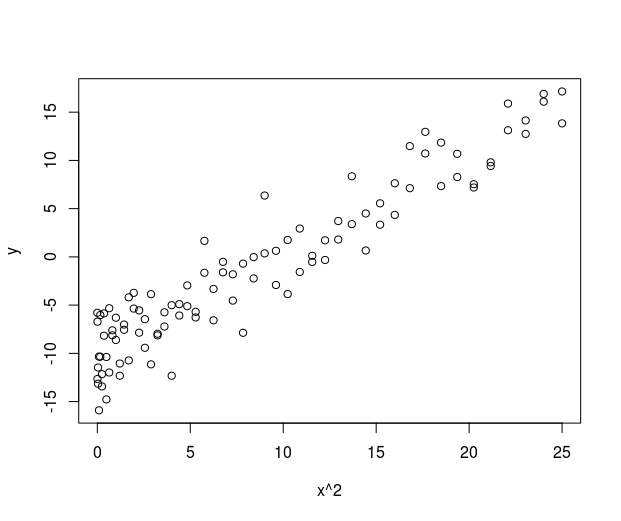
\includegraphics[width=70mm]{/home/t/UVa/all_teaching/3120_slides/12/12.1/pics/Rplot02.png}
\end{center}


\end{frame}
%----------------------------------------------------------------------------------------
\begin{frame}
\frametitle{Logistic Regression}

So far we've assumed $Y$ is normal. In particular it is continuous and takes values on $\mathbb{R}$. 
\newline

What if $Y \in \{0,1\}$? If $Y$ is a Bernoulli rv, it's average $p \in [0,1]$, but $\beta_0 + \beta_1 x$ might not be...
\pause
\newline

Well we have to transform $p$ a bit. We still assume it depends on $x$. So let's call it $p(x)$ now.
\[
\log \left( \frac{p(x)}{1 - p(x)} \right) = \beta_0 + \beta_1 x
\]
\end{frame}
%----------------------------------------------------------------------------------------
\begin{frame}
\frametitle{Logistic Regression}

$\log(p/(1-p))$ is called the \textbf{logit function}. You can interpret it as the log of the odds ratio.
\newline

Its inverse is called the \textbf{logistic (or sigmoid or sigmoidal logistic, etc.)} function. You can write it like this 
$$
\frac{e^x}{1 + e^x} = \frac{1}{1 + e^{-x}}.
$$
\newline

\end{frame}
%----------------------------------------------------------------------------------------
\begin{frame}
\frametitle{Logistic Regression}

So we can write our logistic model two different ways:
\[
\log \left( \frac{p(x)}{1 - p(x)} \right) = \beta_0 + \beta_1 x 
\]
or
\[
p(x) = \frac{e^{\beta_0 + \beta_1 x}}{1 + e^{\beta_0 + \beta_1x}}
\]


Note that we don't have any additive noise or $\epsilon$s around 
\end{frame}

\end{document} 
